\subsection{Anwendungsbereiche}
\subsubsection{Recherchegrund}
Wir wollen wissen, ob und welche Abwasserkraftwerksysteme bereits bestehen. Gibt es  Systeme für die Energiegewinnung via Abwasserturbinen in Hochhäusern? Wie sieht deren Markt aus?
\subsubsection{Ergebnisse}
Grosse Wasserkraftwerke (ca. 100\si{MW}) brauchen viel Platz (grosse Dämme und lange Kanäle) und haben einen unvorhersehbaren Effekt auf Flora und Fauna. Deshalb wird die Entwicklung und Realisierung von Kleinkraftwerken (ca. 100\si{kW}) wichtiger. Die Entwicklung von Abwasserkraftwerksystemen spielt dabei eine grosse Rolle. Folgende erforschte und oder bestehende Systeme konnten gefunden werden:
\paragraph{In Kanalisation zwischen Stadt und Kläranlage}
Wenn in den Abwasserrohren zwischen einer Stadt und deren Kläranlage ein hydraulisches Potential vorliegt, könnte dieses durch Turbinen genutzt werden. Bereits 1992 wurde in Le Châble eine Pelton-Turbine eingesetzt, um das Abwasser vom höher gelegenen Ferienort Verbier zu nutzen \cite{waterworld}.
In Japan wurde in der Gegend des Toyogawa-Flussbeckens untersucht, ob hydraulische Potentiale in den Abwasserrohren bestehen \cite{uchiyama2016feasibility}. Zudem wurden drei kleine Turbinen mit unterschiedlicher Beschaufelung auf Verstopfung durch Fremdmaterial untersucht. Die Studie schliesst mit einem positiven Ergebnis.
\paragraph{In Abfluss von Kläranlagen}
\textit{``Electricity is the second largest operating cost at WWTPs} [Kläranlagen]\textit{, representing 25 to 40\% of the total operating budget.''} \cite[2]{NYSERDA}
Viele Kläranlagen (z.Bsp. Aquarion Water Co (USA) und North Head WWTP (AUS)) sind bemüht, ihre Energiekosten zu reduzieren. In Australien wurde dies in einem Pilotprojekt bereits realisiert, indem das hydraulische Potential genutzt wurde, das zwischen der Kläranlage und dort, wo das gereinigte Wasser hinfliesst, besteht. \cite{powermag} Das dort verwendete Turbinensystem (Flow-to-Wire) \cite{rentricity} wurde von der amerikanischen Firma Rentricity hergestellt. Der Vorteil von dieser Variante ist, dass das Problem der Verstopfung duch das bereits gereinigte Wasser ausbleibt.
LucidPipe \cite[4]{LUCIDPIPE}, ist ein anderes, von Lucid Energy entwickeltes System, das in Oregon und Kalifornien innerhalb von Trinkwasserleitungen verwendet wird. Es wird erwähnt, dass ein grosser Wasserstrom (53 Mio. Liter pro Tag) nötig ist, damit sich eine Installation lohnt. \cite[4]{LUCIDPIPE}
\paragraph{In Hochhäusern}
Es wurde nur ein Pilotprojekt gefunden, wo eine Abwasserturbine für die Anwendung innerhalb von Gebäuden entwickelt wurde \cite{newatlas}. Der Entwickler Tom Broadbent, unten in der Abbildung \ref{fig:turbineTomBroadBent} zu sehen, sagt \textit{``}[...] \textit{the electricity generated by the HighDro Power can either be used in the building to save around GBP925-per-year (approx US\$1,410) or sold back to the national grid on a buy-back tariff.''} \cite{newatlas}
\newpage
\begin{figure}
\centering
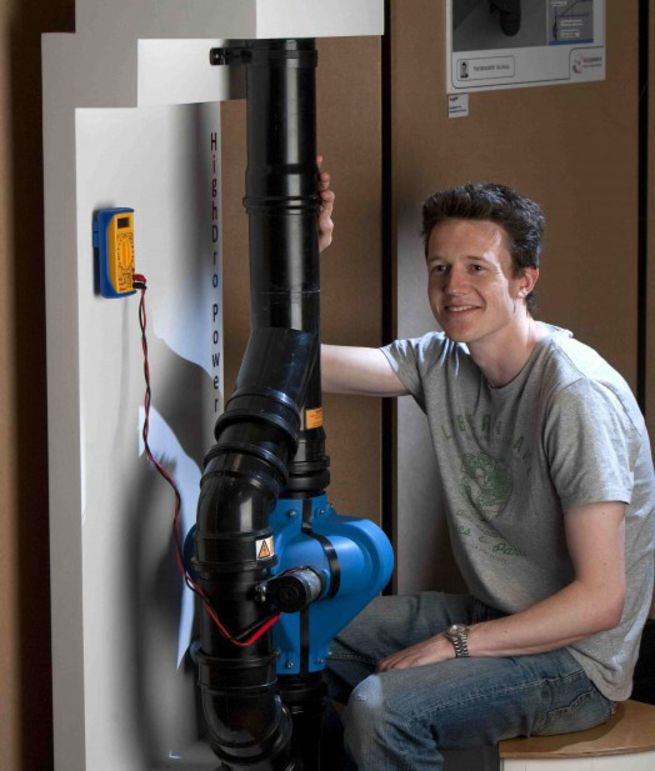
\includegraphics[width=6cm]{highDro.jpg}
\caption{Tom Broadbent und HighDro. \cite{newatlas}}
\label{fig:turbineTomBroadBent}
\end{figure}
\paragraph{Andere Anwendung in Hochhäusern}
Die Trinkwassersorgung der obersten Stockwerke eines Hochhauses erfordert viel Druck (6-8 Bar). Weil dieser Druck für die unteren Stockwerke zu gross ist, müssen Druckreduzierventile eingesetzt werden. Dabei bleibt viel Energie ungenutzt. In Hong Kong testet die Firma Arup bereits in zwei Hochhäusern eine andere Lösung: Statt Druckreduzierventile werden Turbinen verwendet \cite{nytimes}. Als Gründe für ein mögliches Scheitern dieser Lösung wird das Preis-Leistungs-Verhältnis genannt:
\textit{``Small-scale systems cannot easily generate enough power to justify their cost to large developers. The price per kilowatt-hour of generating power can be five times as high as simply buying it from the grid.''}\cite{nytimes}
\subsubsection{Fazit}
Der Markt beschränkt sich auf die Anwendungsbereiche, wo ein grosser Wasserfluss besteht, also in Zu- und Abflussrohren von Kläranlagen. Erfolgreiche Hersteller für Abwasser-Turbinen in Gebäuden gibt es keine, da das Preis-Leistungs-Verhältnis der bisher entwickelten Turbinen wegen geringem Wasserfluss und hohen Installationskosten ungenügend ist. Von fünf gefundenen Projekten resp. Produkten fiel nur eines in unseren Bereich (Abwasserleitung in Gebäude): Das HighDro (unten rot markiert). Es wäre also möglich, in dieser Nische ein neues Produkt einzuführen, wenn es den Anforderungen genügen kann.

\definecolor{highliteMe}{rgb}{1,0.4,0.4}
\begin{tabular}{l l l l}
 \textbf{Firmenname} & \textbf{Objekt} & \textbf{Anwendungsbereich} & \textbf{Anwendungsort}\\	
  \hline	
  \textbf{Lucid} & LucidPipe & Trinkwasserleitung & Oregon, California \\
  \textbf{Arup} & V-axis spherical turbine & Trinkwasserzuleitung Haus & Hong Kong\\
  \textbf{VA Tech} & 700\si{kW} Pelton & Abwasserkanal & Le Châble\\
  \textbf{Hydro} & & &\\
  \textbf{Rentricity} & Flow-to-Wire &  Abfluss Kläranlage & Sydney\\
  \rowcolor{highliteMe}
  \textbf{n. a.} & HighDro & Abwasserleitung in& n. a.\\  
  \rowcolor{highliteMe}
  & & Gebäuden & \\
\end{tabular}
\clearpage 
